\scanpage{150}\mspage{24}
Revenons à la majoration cardinale des $X_\alpha(f)$, où $f:X\unsure{\mathrel{\text{---}}|\longrightarrow}Y$ \deleted{dans} ds $\mathrm{Fl}^{\unsure{s|B}}M$ i.e. $X,Y\in\mathrm{Filt}^s$. On suppose en plus $C_0\subset\deleted{\mathrm{Filt}}\mathrm{Fl}^rM$,
\deleted{\unsure{et}}
\[
\left\{\begin{aligned}
&C_0\subset\mathrm{Fl}^rM=\mathrm{Fl}\,M^r,\qquad(f:X\mathrel{\text{---}}Y)\in\mathrm{Fl}^sM\quad\text{i.e. }X,Y\in\mathrm{Filt}^s\\
&s\ge r
\end{aligned}\right.
\tag*{(3.10)}
\]
\deleted{\unsure{OBS} \unsure{pour} $C_0$, \inserted{\unsure{compté}} \unsure{mod.|modulo} \unsure{réun.|près|classes} \unsure{disjte|d'isom.}}
\[
\deleted{\mathrm{Card}\,\Delta(C_0,f)\le\mathrm{card}\,M^r_{/X}\times\mathrm{Card}\,M^r_{/Y},}
\]
Il y a une difficulté \unsure{idiote|ici}, c'est que \deleted{\unsure{de}} $M^r$ est équivalente à une petite catégorie, mais n'est pas elle-même petite. Même si $C_0$ ne \unsure{contenant|contenait} qu'une seule classe d'isomorphie de flèches de $M^r$, son cardinal pourrait être (pour $r$ fixé) arbitrairement élevé. Aussi dans ce qui suit, je \inserted{\unsure{dois|vais}} supposer \deleted{que le} \inserted{la condition} \deleted{\unsure{nb|est} \unsure{d'éléments|d'ailleurs} \unsure{cardinal} de \unsure{C|C_0}} de ``non \unsure{pléthoricité|pléthorité}'' cardinale pour $C_0$
\[
\begin{aligned}
&\forall i\in C_0,\ \deleted{\unsure{l'ens|désignant}}\inserted{\text{désignant}}\ \text{par }C_0(i)\text{ l'ens des}\\
&\deleted{\unsure{d'}}i'\in C_0\text{ telles que }i\simeq i'\text{ dans }\mathrm{Fl}\,M,\ \text{j'impose}\\
&\text{que}\quad\mathrm{card}\,C_0(i)\le2^{(r^{\pi_0})}\quad\text{(ce qui est \inserted{aussi}}\\
&\text{\inserted{visiblement la} majoration pour le cardinal de }\widetilde{\underline{\mathrm{Fl}}^rM}=\widetilde{\underline{\mathrm{Fl}}\,M^r})
\end{aligned}
\tag*{\unsure{(3.1b)|(3.11)}}
\]
\margin{$\deleted{\mathrm{card}}\inserted{\mathrm{card}\,C_0\le}\left(2^{(r^{\pi_0})}\right)^2=\mathrm{card}\,2^{r^{\pi_0}}$.}
Cela \unsure{entraîne|entraine} donc que l'on \unsure{a}
\[
\mathrm{card}\,C_0\le2^{(r^{\pi_0})},
\tag*{(3.12)}
\]
qui est équivalente à (3.1b) (moyennant $C_0\subset\mathrm{Fl}^rM$, postulé dans (3.10)).
Il s'ensuit \inserted{par (3.8)} que l'on a
\[
\mathrm{card}\,\Delta(C_0,f)\le
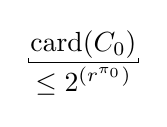
\begin{tikzpicture}[baseline=(t.base)]
\node[inner sep=1pt] (t) at (0,0) {$\mathrm{card}(C_0)$};
\draw (-0.7,-0.18)--(-0.7,-0.23)--(0.7,-0.23)--(0.7,-0.18);
\node[anchor=north,inner sep=1pt] at (0,-0.25) {$\le2^{(r^{\pi_0})}$};
\end{tikzpicture}
\cdot\unsure{s|2|8}^{(r^{\pi_0})}\cdot s^{(r^{\pi_0})}\le s^{(r^{\pi_0})}.
\]
D'autre part, les $X_D$ dont on prend la somme amalgamée sous $X$, pour obtenir $X_1(f)$, sont dans $M^s$, si on fait l'hypothèse \unsure{suivante}
% archive sheet number: 149
